\documentclass{article}
\usepackage{geometry}
\usepackage{graphicx}

% Path to graphic images
\graphicspath{ }

% Title
\title{Wifi Connected Chess Boards}
\author{Nick Kraus, Kyle Jameson, Maurice Wallace, Mark Mauriello}
\date{\today}

% Margins
\geometry{letterpaper, portrait, margin=.75in}

\begin{document}

\maketitle

%-----------------------
%		Background		
%-----------------------

\section*{Background}
\indent

Chess and its predecessors have been played for well over 1000 years, and yet the game has only seen serious development in the 20th and 21st centuries. This came with the establishment of the World Chess Federation, advancements to chess theory, and the developments of computer analysis and artificial intelligence.\\
\indent

As new technologies appeared it has become easier and easier to enjoy an engaging match of chess with a friend. The invention of the internet allowed people to play with each other across the world, and the advancement of computers made it no longer necessary to have a human opponent.\\
\indent

As technology progresses it will be interesting to see where the future of chess goes. While technology continues to become an intricate part of games, including chess, there is still nothing quite like sitting down with a friend and playing a physical game of chess, even if that isn't always an option.

%-------------------------------
%		Project Summary			
%-------------------------------

\section*{Project Summary}
\indent

The goal of this project is to create a set of chess boards which can play against each other wirelessly over the internet. These chess boards will wait for the player to move a piece and finish his turn, and then move the corresponding piece on the opponents chess board. This will allow the realism of a physical game of chess while still allowing people from distant locations to play against each other.\\
\indent

The chess board can also have the option to play against people who are playing online on their computer, by communication with a server, and relaying the opponents moves back to the physical chess board. This ability allows for many more matchmaking opportunities to the user of the chess board, as playing is no longer limited to others who own such a board.

%-----------------------------------
%		Project Implementation							
%-----------------------------------

\section*{Project Implementation}
\indent

The implementation of our project is made up of 3 main groups, the mechanical system, the embedded electronics system, and the software web interface. Each system consists of multiple other parts, but the systems are in general independent of each other except for very well defined interfaces. This separation of function will allow for work to be completed on different areas of the project simultaneously. Below the implementation of the chess boards is outlined.\\

\begin{itemize}
	
	\item Mechanical System

	\begin{itemize}

		\item The chess pieces contain neodymium magnets underneath, to allow movement and piece detection.
		\item An electromagnet underneath the playing surface controls the movement of chess pieces.
		\item An x-y gantry (in an h-bot configuration) controls the position of the electromagnet.
		\item The x-y gantry is driven by two stepper motors and accompanying stepper motor drives.
		\item Limit switches should be included to help the system self-calibrate before running.
		\item The embedded system directly controls the stepper motor drivers and power supply of the electromagnet.

	\end{itemize}

	\item Embedded System

	\begin{itemize}

		\item Contains an ARM Cortex-M microcontroller as the main processor for the chess board.
		\item Contains an ESP8266 WiFi module to communicate with the web interface.
		\item The MCU will:

		\begin{itemize}

			\item Detect the position of chess pieces by reading hall effect sensors under the playing surface.
			\item Control the position of the gantry by interfacing with the stepper motor drivers.
			\item Store information about the current state of the chess game.
			\item Make sure the next move is legal, and warn the player if not.
			\item Control a UI, allowing the player to finish his move, start a new game, view a game clock and other options.

		\end{itemize}

	\end{itemize}

	\item Web Interface

	\begin{itemize}

		\item The web interface will expose an API through which the WiFi module will communicate.
		\item The web interface will host a chess server which the boards will interact with.
		\item The chess server will store minimal information about the state of the chess game, allowing the embedded system to perform most of the computations.
		\item The web interface can be used with a software application instead of a WiFi chess board.

	\end{itemize}

\end{itemize}

\section*{Budget}
\indent

The project is designed to be released as an open source project upon completion, therefore competitive pricing of the design isn't crucial to its success. However we are hoping to have a single unit cost of approximately \$100, with a prototype unit cost of approximately \$200. This amount will go towards covering the cost of all the mechanical and electrical components, including microcontrollers, the WiFi module, other electronic components, stepper motors, and the gantry system.

\section*{Conclusion}
\indent

As technology continues to exponentially increase in power and pervasiveness in our every day lives, more and more tasks will turn to software solutions. Yet there is always something familiar and satisfying about physical interfaces to a system, even if that underlying system isn't physical itself. The WiFi Chess Board is a unique implementation of a very well used idea in todays day and age, and a great way to keep the traditions of this enticing game alive for many more years. With a good balance between hardware and software design this project would be very appropriate for a multi-disciplined group of engineers.

\clearpage

\section*{Diagrams}

\centerline{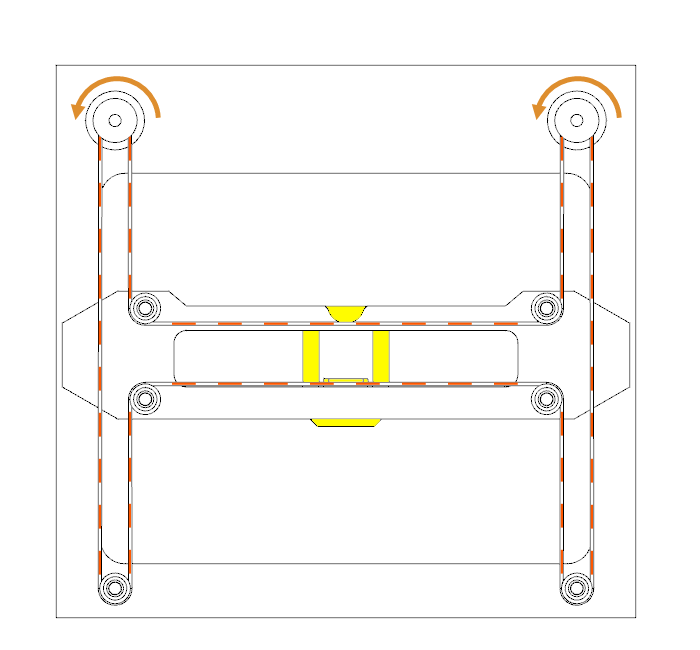
\includegraphics[scale=.5]{hbotimage}}
\centering

Figure 1: An x-y gantry in a h-bot configuration. Moving both motors in the same direction results in movement on the x-axis, while moving both motors in opposite directions results in movement on the y-axis.

\end{document}